\chapter{Results}
\label{ch:results}

\section{Automatic bot detection}

\subsection{Friends graph}
In Figure \ref{fig:user-graph-louvain}, you can see the visual representation of the graph produced with ForceAtlas 2 layout algorithm. In various bright colours, the largest clusters (clusters that contain more than 2\% of the users in the dataset) are shown. The remaining clusters are coloured grey.

\begin{figure}
	\centering
	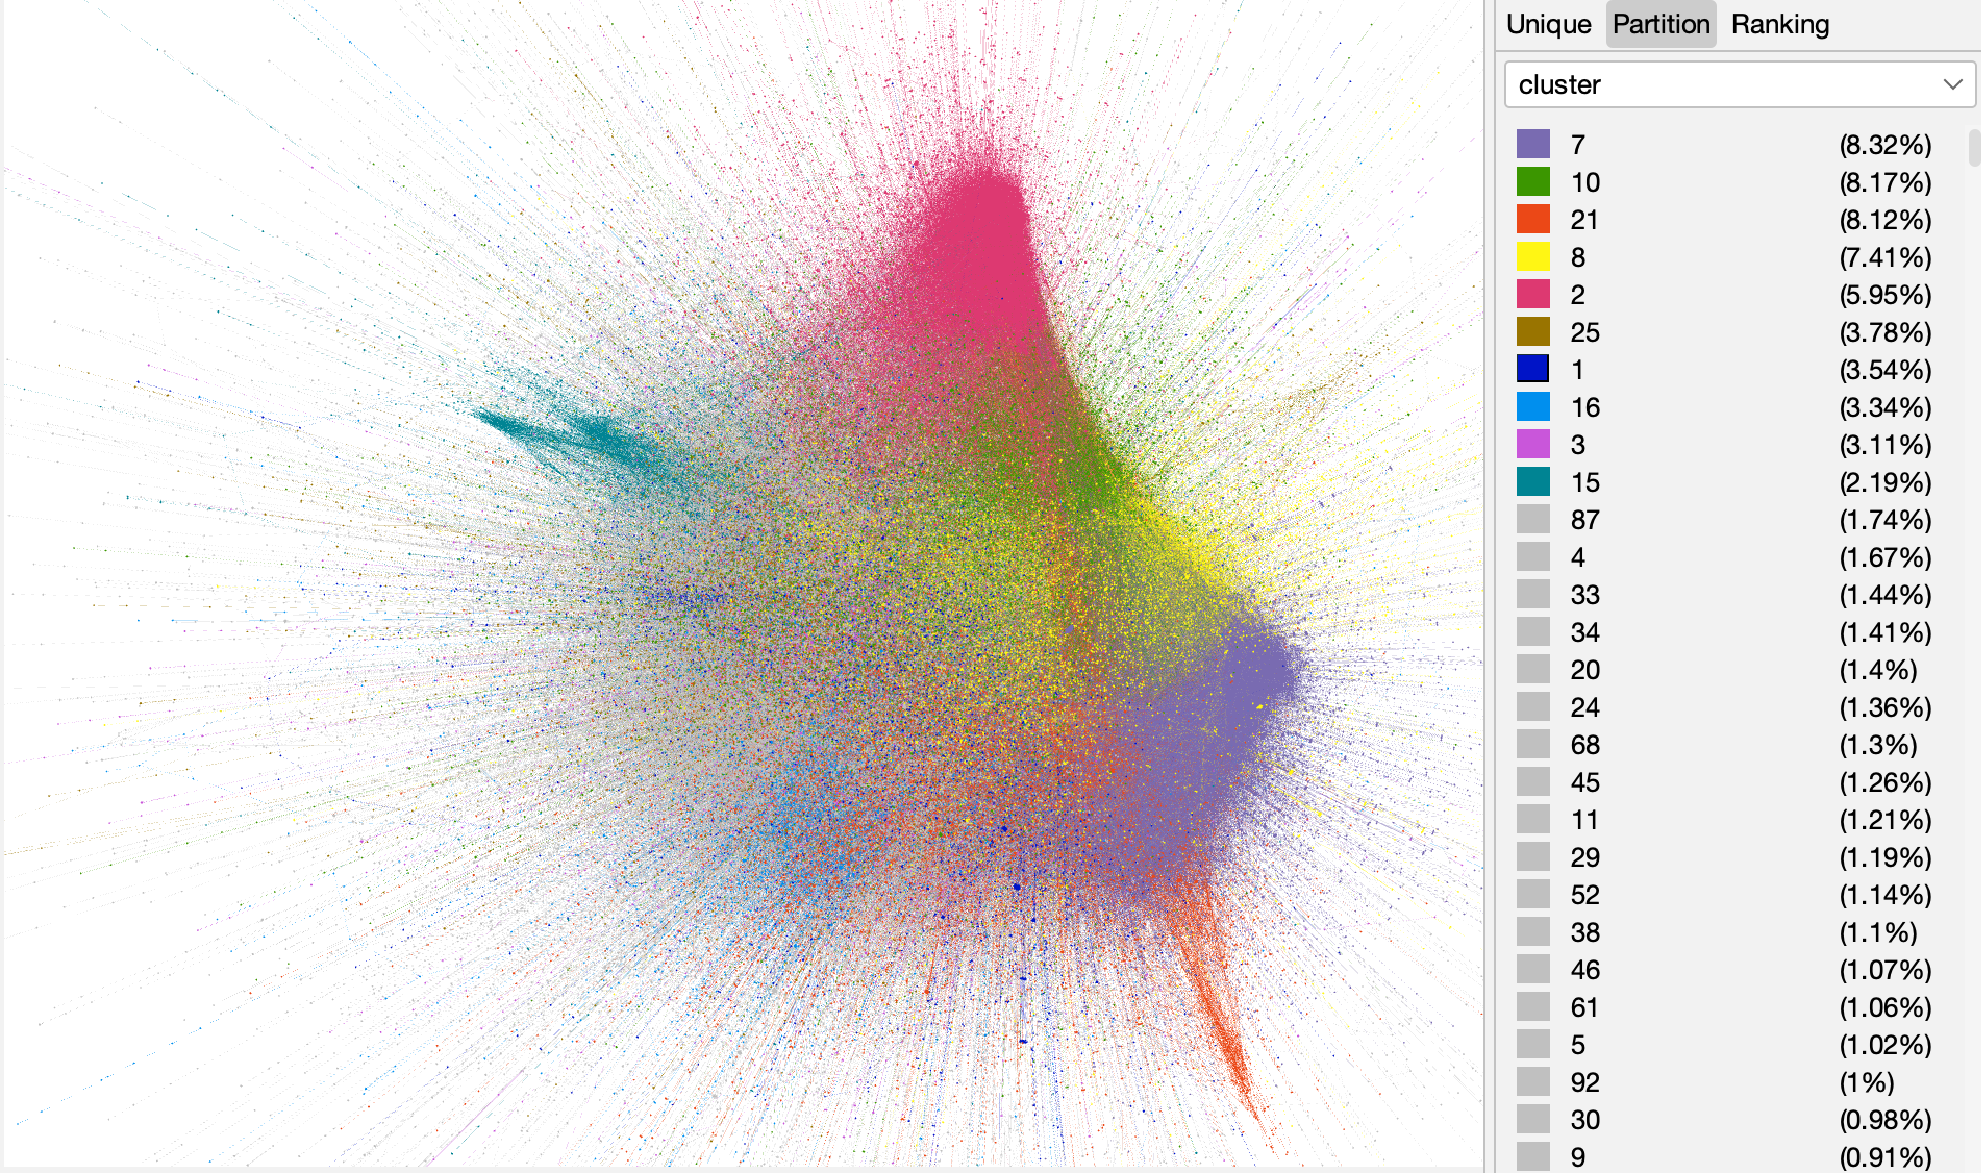
\includegraphics[width=1.0\linewidth]{Thesis/Images/user-graph-louvain-clustered.pdf}
	\caption{User graph clustered with Louvain algorithm, ForceAtlas 2 layout}
	\label{fig:user-graph-louvain}
\end{figure}

Even though the clusters can be visually identified, they are quite tightly
connected. In Figure \ref{fig:user-graph-louvain} we can notice at least seven major clusters: clusters number 7 (lilac), 10 (green), 21 (orange-red), 8 (yellow), 2 (crimson), 16 (lighter blue), 15 (aquamarine). These clusters present a great interest for further investigation because they are quite large compared to the rest of the clusters and are the most visually separable from the rest. The clusters 25 (brown), 1 (dark blue) and 3 (pink) are also visible but are not so clearly separable from one another.

Next, we explore the distribution of users that we definitely know or suspect to be real humans, throughout the graph. These users include verified users and ``friends and friends of friends'' users.

For the verified users, it is known for sure that they are real humans: they undergo a document check before receiving the ``verified'' label. The placement of verified users on the user graph is shown in Figure \ref{fig:users-distribution-friends-graph} in bright green colour.

\begin{figure}
	\centering
	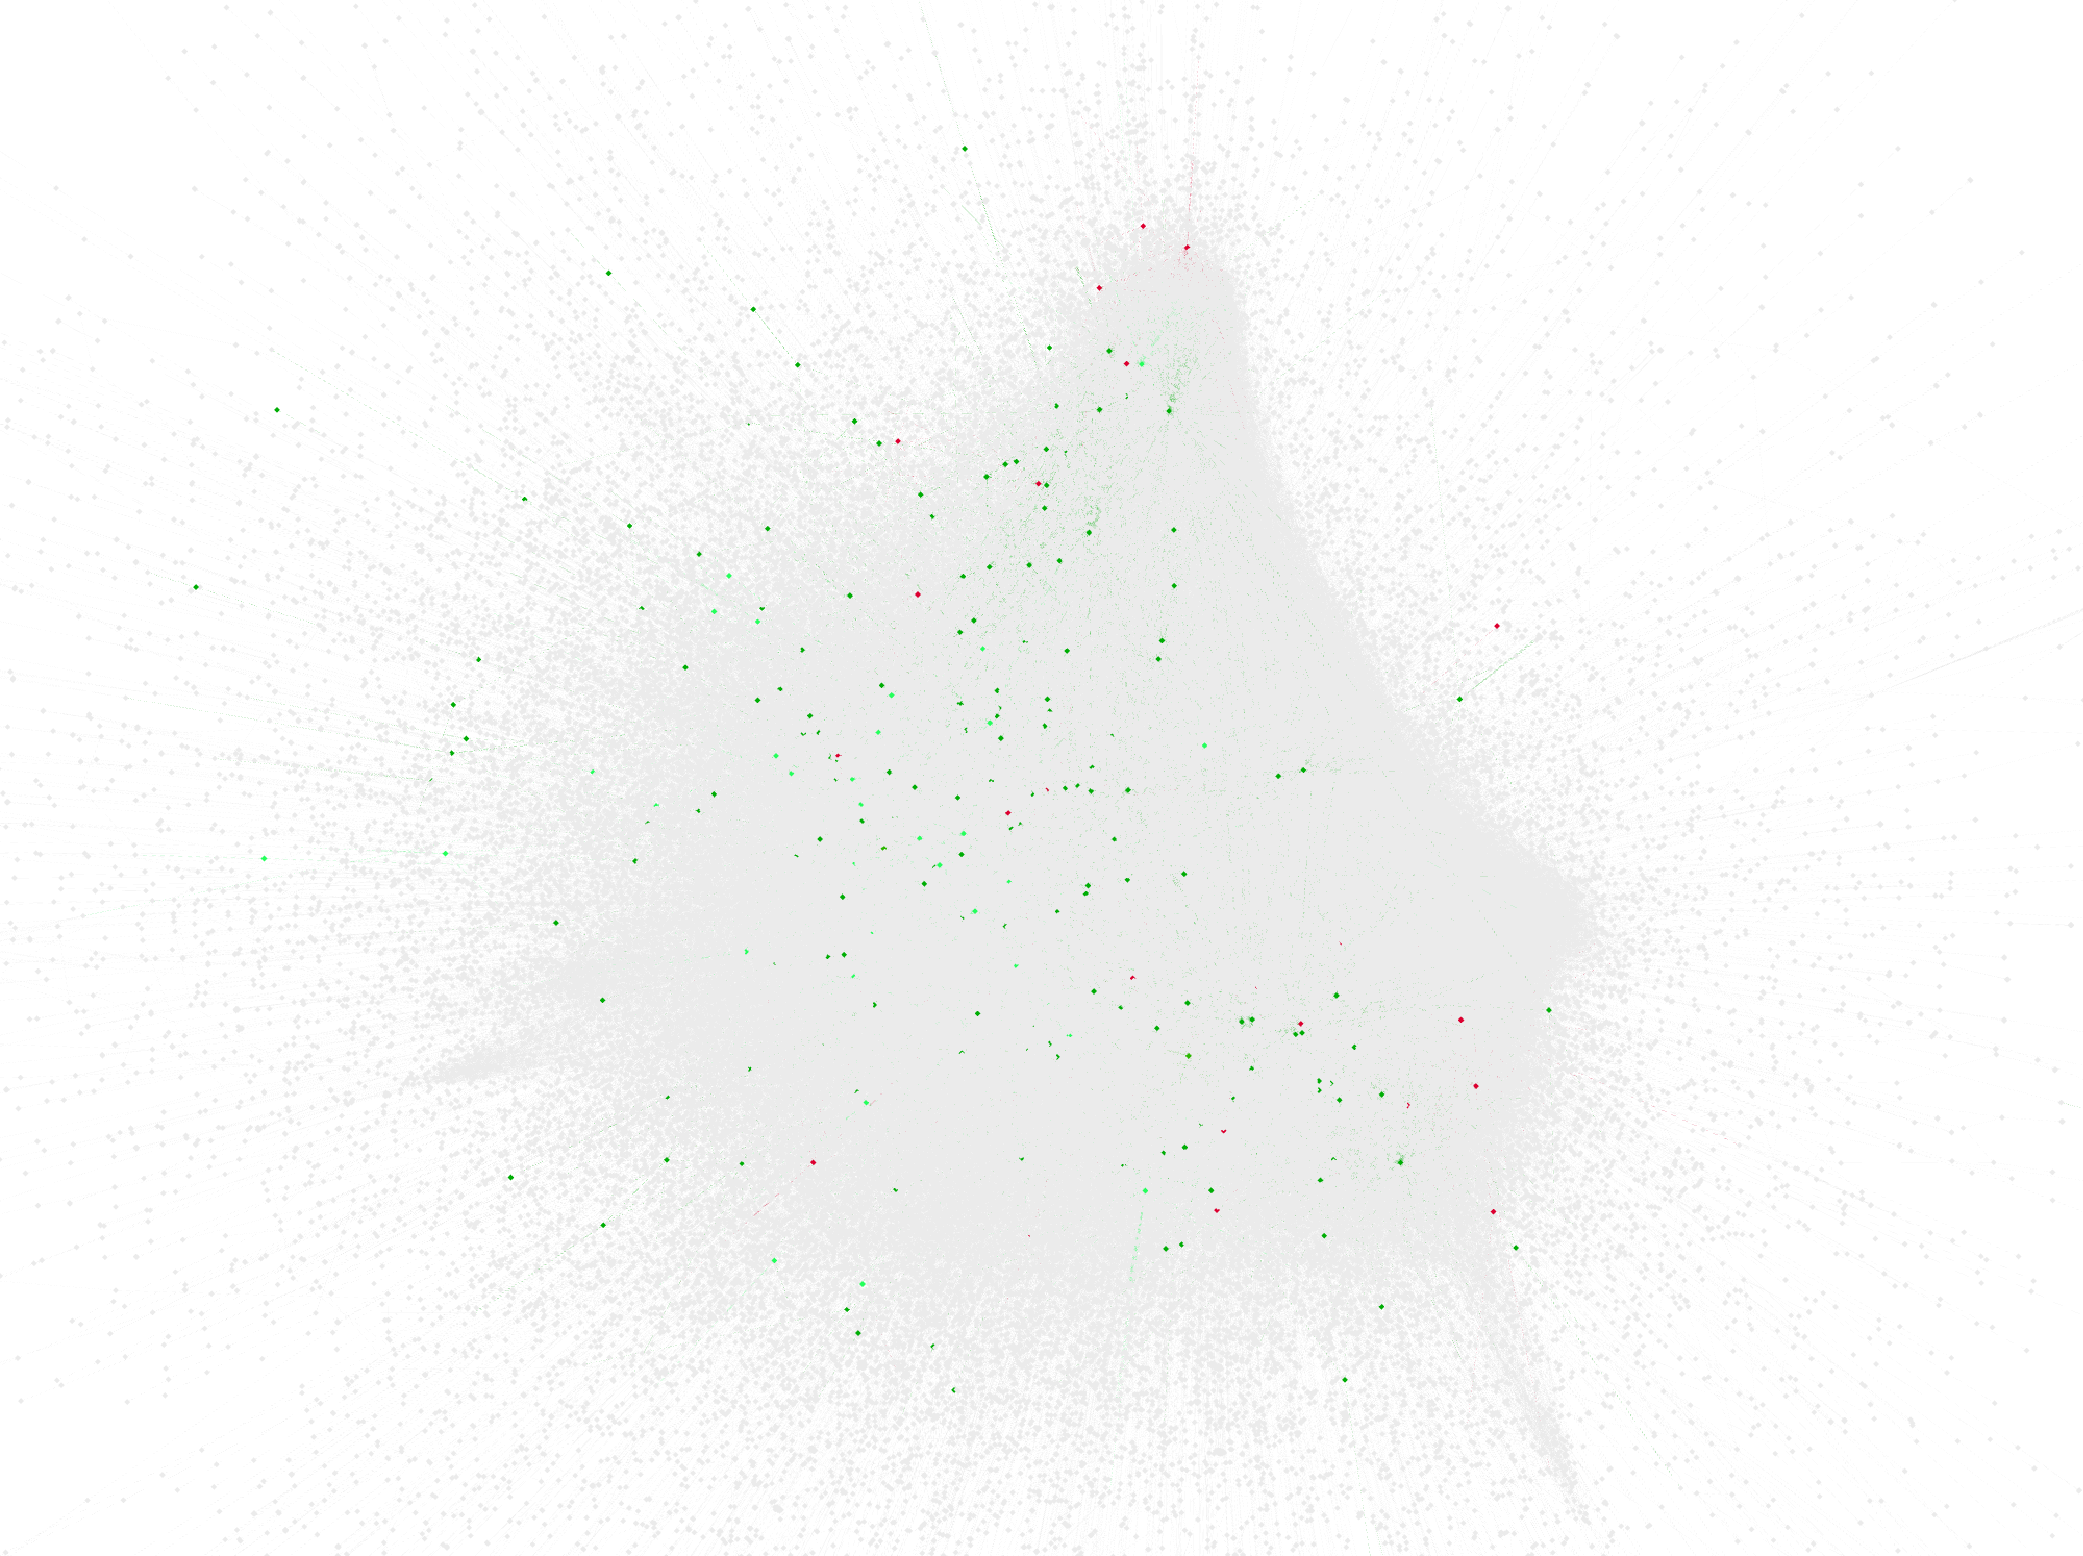
\includegraphics[width=1.0\linewidth]{Thesis/Images/users-distribution-friends-graph.pdf}
	\caption{User graph with verified (bright green), banned (red) and friends (light green) users}
	\label{fig:users-distribution-friends-graph}
\end{figure}

It can be clearly seen that the position of all verified users is skewed to the left, with very few of them on the right side of the graph. Thus, the concentration of users whom we definitely know to be human is zero in almost all noticeable clusters that are separable from the other ones. Taking a look at the major clusters mentioned above, we notice that in clusters 7, 15 and 3 there are no verified users. Clusters 1 and 2 contain only one verified user each. At the same time, the major clusters 10, 21, 25 contain much more verified users.

Next, the concentration of ``friends and friends of friends'' of the thesis’ author is explored. In Figure \ref{fig:users-distribution-friends-graph}, we can also see a skew to the left, with very few users on the right side of the graph. A lot of such users belong to the major clusters mentioned above, e.g. 6 users belong to cluster 1, 29 users to cluster 2. Cluster 15 does not contain any such users.

It is crucial not only to identify the position of potential real humans on the graph, but that of bots, too. The only probable indicator that we have for bots is the ``banned'' status from VKontakte API. The banned users are displayed as right dots in Figure \ref{fig:users-distribution-friends-graph}.

It is possible to divide all the clusters into three categories:
\begin{itemize}
    \item Clusters that contain a high number of banned users and low number of verified and ``friends of friends'' users. These clusters are highly likely to consist of bots.
    \item Clusters that contain a low number of banned users and high number of verified and ``friends of friends'' users. These clusters are highly likely to consist of real human users.
    \item Clusters that either do not contain verified, friends and banned users, or contain them in an equal proportion. These clusters are unidentified by the model, by default we assume they are human.
\end{itemize}

To identify the thresholds applied to the number of banned and verified users in a cluster, we adhere to a rule that the number of bots in our network should be around 1\%, as previous research shows that is the typical number for VKontakte\cite{vkBotPercentage}.

The logic of applying the thresholds to the clusters was the following:
\begin{itemize}
    \item If the percentage of banned users in a cluster is higher than the ‘banned\_threshold’ that equals 0;
    \item And the percentage of verified users in a cluster is lower or equal than
    the ‘verified\_threshold’ that equals 0.0005;
    \item And the percentage of ``friends and friends of friends'' users is lower or equal than the ‘friends\_threshold’ that equals 0.0025;
    \item Then the cluster is identified as a potential bot cluster. Otherwise, it is a human cluster by default.
\end{itemize}

By choosing the thresholds for the level of banned, verified and friends users,
the following results are achieved. 6 clusters are identified as potential bot clusters (clusters number 1, 3, 7, 24, 35, 158), or ``suspicious'' clusters. These 6 clusters contain 16,3\% of the total number of users. These 16,3\% of users have left 22,3\% of the total comments saved in the database.

We next compare the predictions of the model to the results of labelling and compute the key metrics for the model. The values of these metrics are the following:
\begin{itemize}
    \item Accuracy: 64.29\%;
    \item Precision: 25.00\%;
    \item Recall: 33.33\%.
\end{itemize}

As we can see, the performance characteristics of this model are unsatisfactory. Changing the threshold values did not improve the metrics. We next hypothesise that the clusters in the user network built on friendship relations are too big and do not allow for the precise identification of bots. In order to build more granular clusters, a different method is needed that allows uncovering hidden connections between users that are not as obvious and widespread as friendship relations.

\subsection{URL sharing}

The final user network contains 986 nodes connected with 1668 edges. Figure \ref{fig:url-sharing} displays the user graph that was obtained with this method. Each node is coloured according to the node's degree. The higher the degree, the darker is the shade of green. Moreover, the clusters in this figure are labelled with identifiers U1-U10. Clusters U1-U6 are ``suspicious'' clusters where the model predicts that the users are bots. The suspicious clusters are easily identified as separate groups of users, usually tightly coupled nodes with a high node degree. Clusters U7-U10 are ``normal'' clusters where the users are supposedly humans. 

\begin{figure}
	\centering
	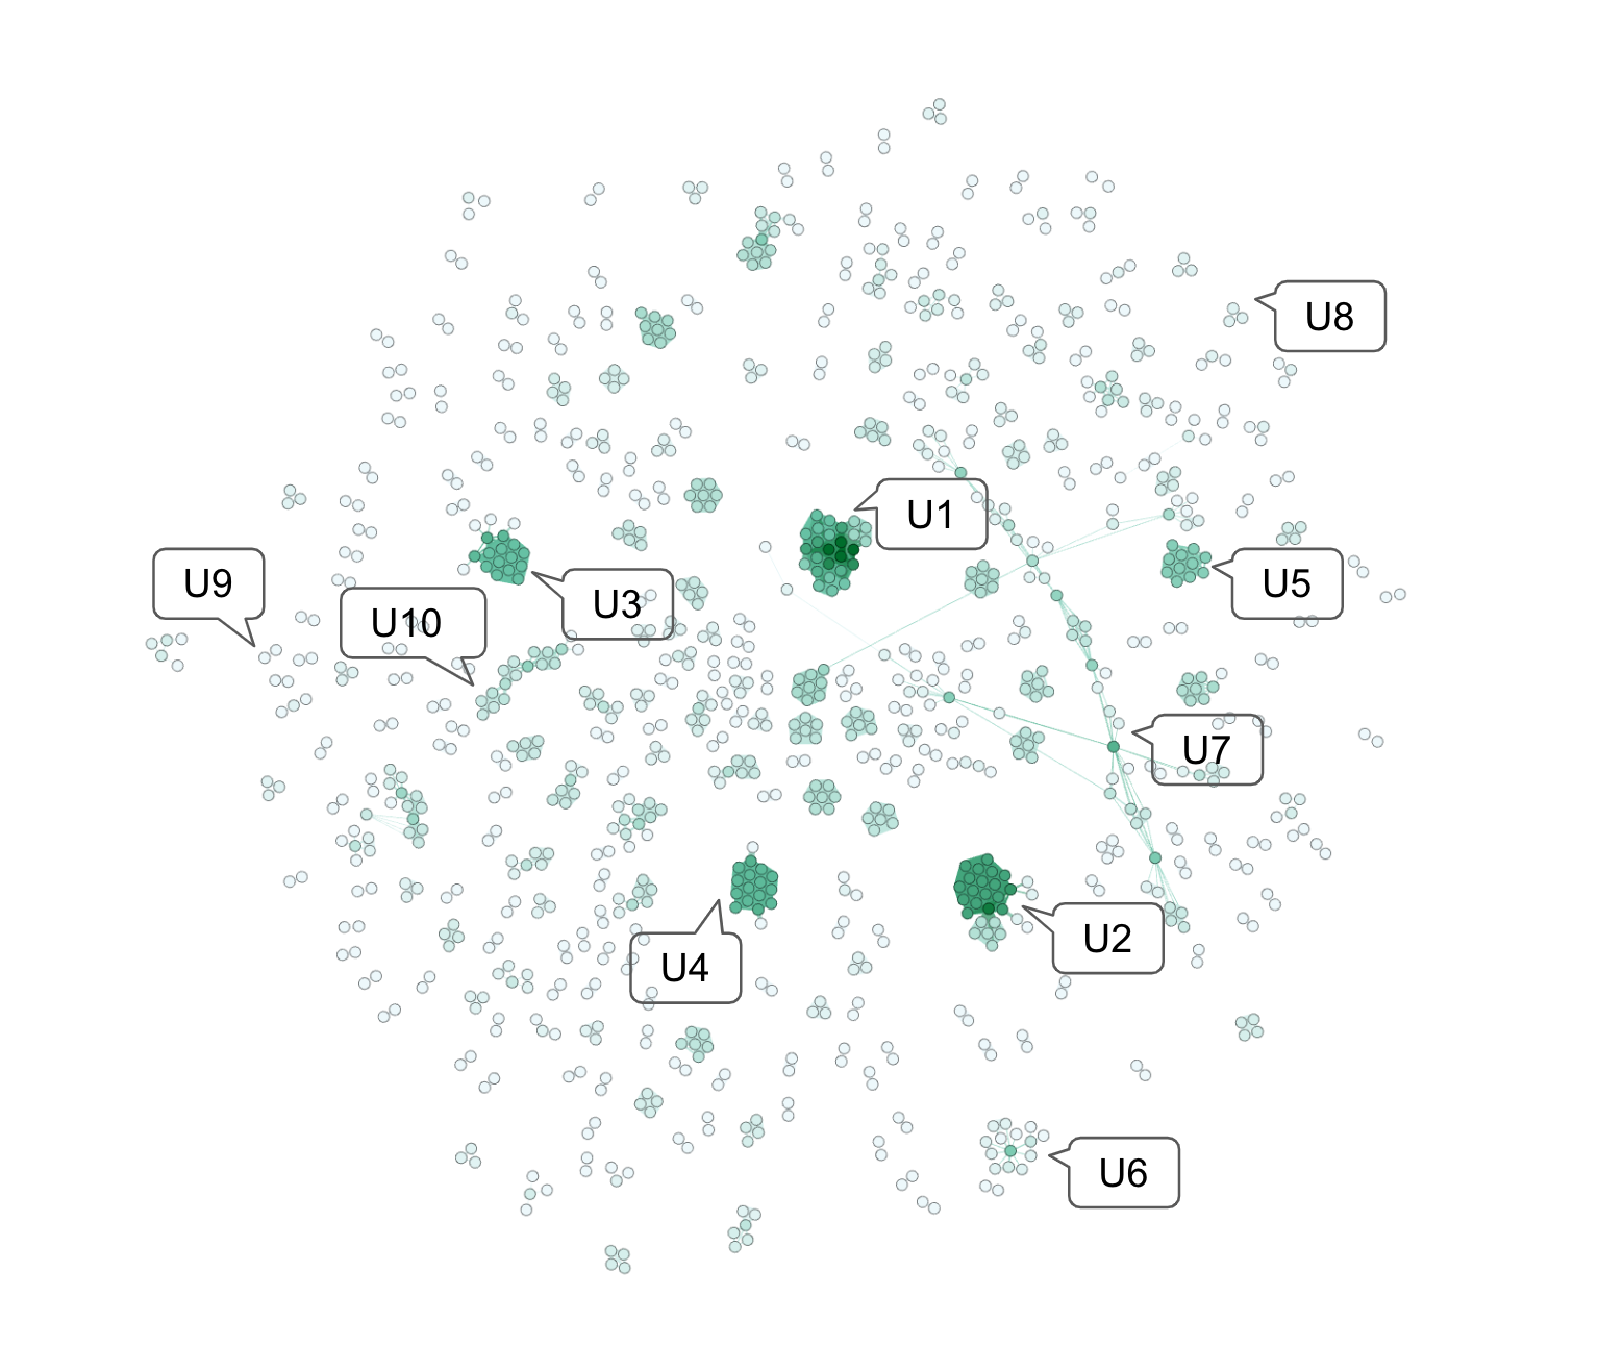
\includegraphics[width=1.0\linewidth]{Thesis/Images/url_sharing_numbered.pdf}
	\caption{User network built with URL sharing  method}
	\label{fig:url-sharing}
\end{figure}

The URL sharing model is evaluated using the labels that were collected in \ref{sec:labelling}. Standard key metrics are calculated to measure model performance:
\begin{itemize}
    \item Accuracy: 85.00\%;
    \item Precision: 83.33\%;
    \item Recall: 90.91\%.
\end{itemize}

Judging by the metrics, the URL sharing model is capable of efficiently identifying bot clusters and human clusters. Dense clusters typically consisting of 5-20 users where users frequently share the same URLs are highly indicative of bots. These clusters are easily separable from the rest of the nodes in the graph and have a distinct structure where either one account is symmetrically connected to all the other accounts or all accounts are tightly coupled between each other. Small clusters with low node degrees and asymmetric clusters, on the opposite, indicate the presence of real human accounts. 

The users from suspicious bot clusters share the same links, the most popular of them are the following:

\begin{itemize}
    \item Cluster U1: Telegram channel, VKontakte and Odnoklassniki group ``dnevniksfronta'' (pro-Russian); negative news about the USA; YouTube video of an explosion in Ukraine; Telegram channel ``redakciya\_channel'' (pro-Russian). 
    \item Cluster U2: the website 200rf.com (a website launched by Ukraine to help Russian families find their relatives that were killed during the conflict; currently not available on the Internet)\footnote{https://www.pravda.com.ua/eng/news/2022/02/27/7326424/}.  
    \item Cluster U3: the Wikipedia article about Russian invasion of Ukraine\footnote{https://en.wikipedia.org/wiki/2022\_Russian\_invasion\_of\_Ukraine}; anti-war YouTube interviews.
    \item Cluster U4: the website 200rf.com, YouTube videos.
    \item Cluster U5: Telegram channel ``warfakes'' (pro-Russian).
    \item Cluster U6: pro-Ukraine Telegram channels and YouTube videos.
\end{itemize}

As we can see, these users most frequently share Telegram channels and YouTube videos, as well as external websites and VKontakte groups. For each cluster, it is possible to identify the attitude towards the Russian-Ukrainian armed conflict and the purpose of URL sharing. 

It is also interesting to find out whether the bots that the URL sharing method has found were detected by VKontakte moderators and banned. To do so, we visualise the user statuses on the user network, showing banned users in bright pink (Figure \ref{fig:url-sharing-banned}). 

\begin{figure}
	\centering
	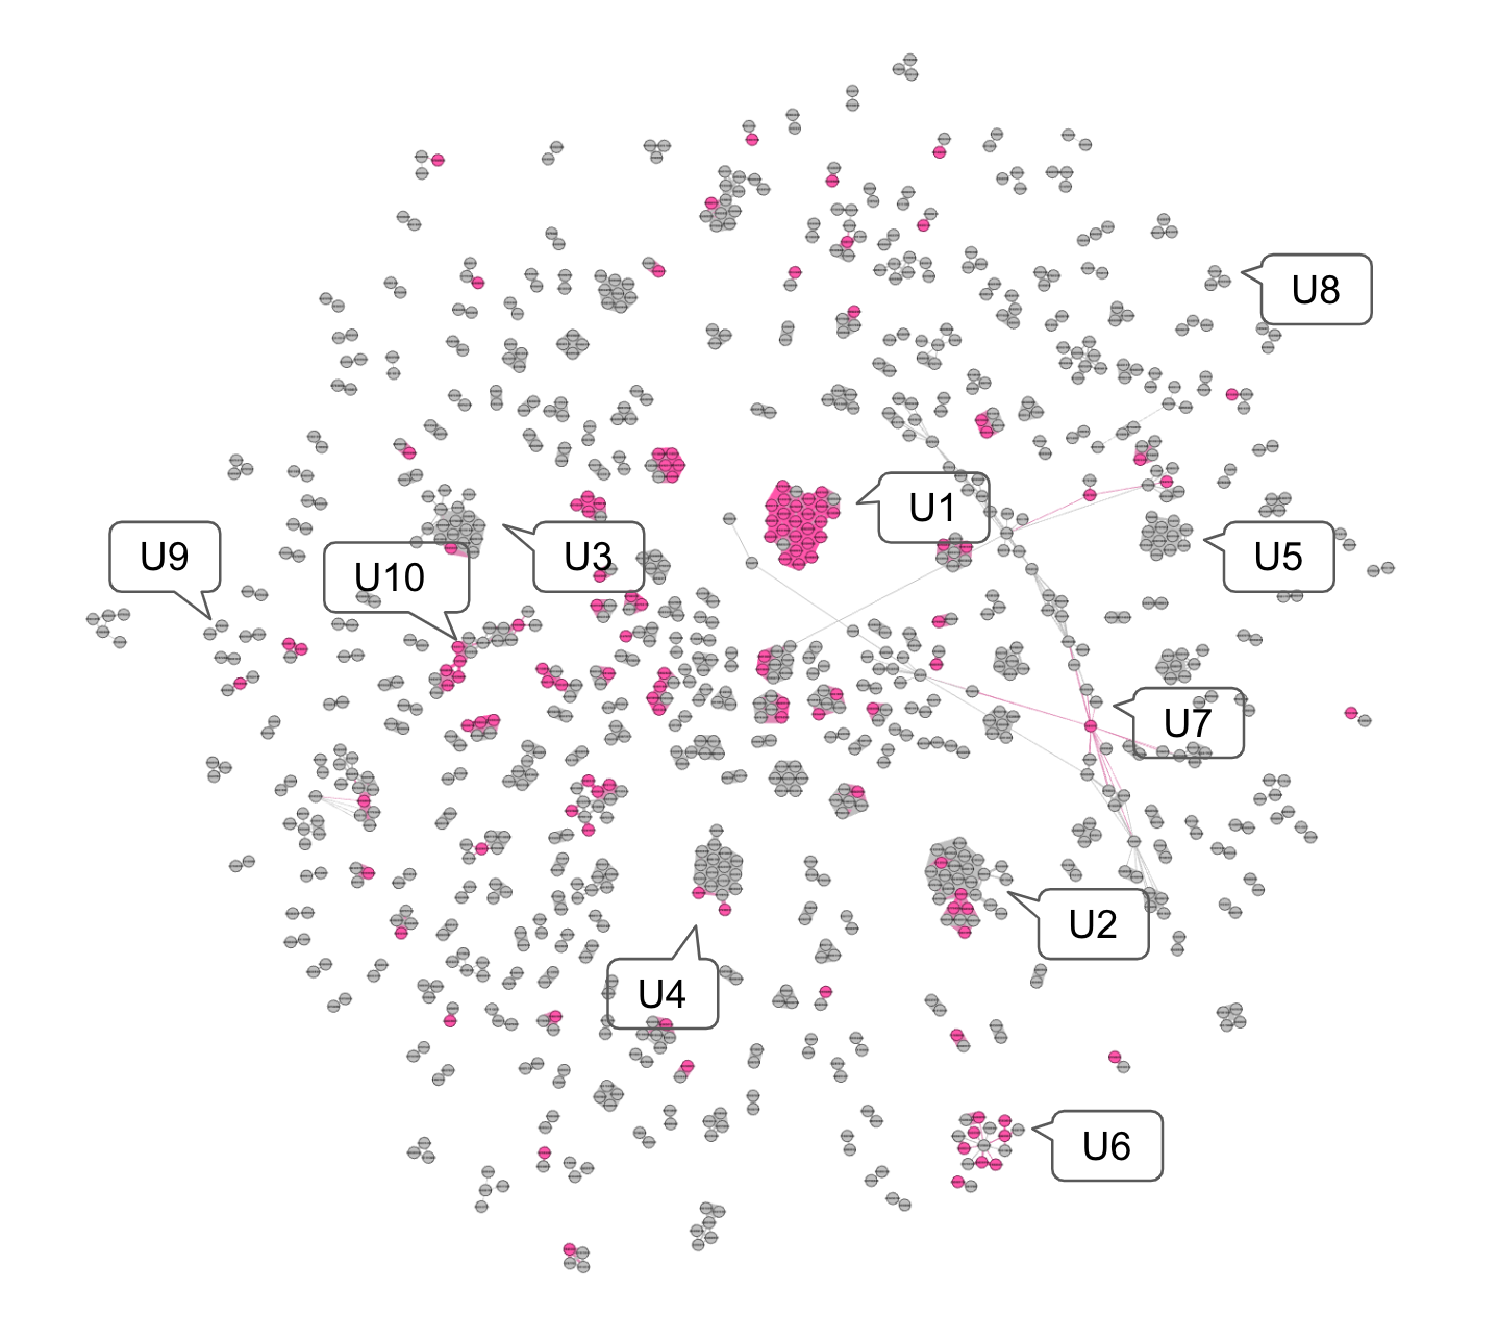
\includegraphics[width=1.0\linewidth]{Thesis/Images/url-sharing-banned.pdf}
	\caption{User network built with URL sharing  method, with banned users in pink colour}
	\label{fig:url-sharing-banned}
\end{figure}

As we can see, some bot clusters contain a high number of banned users (e.g. cluster U1 and U6). This means that users from these clusters were likely banned because VKontakte moderators considered them bots. On the other hand, these clusters contain a few active users that are not banned yet. Moreover, bot clusters U2-U4 contain very few banned users and bot cluster U5 contains none. This means that these bots have escaped being banned on the platform. 

As a result of applying the URL-sharing method, a model able to successfully identify bot and human users was created. The model has high accuracy, precision and recall values and identifies bots that avoided banning on VKontakte. URL-sharing group-based method is both an easy and efficient method of detecting coordinated groups of bots in the discourse about the Russian-Ukrainian armed conflict.


\subsection{Hashtag sequences}
As a result of applying this method, we obtain a user network consisting of 384 nodes connected with 4087 edges. While this graph contains three times less nodes than the URL-sharing graph, the nodes are a lot more connected and form tighter clusters. This can be seen in Figure \ref{fig:hashtag-sequences}.

\begin{figure}
	\centering
	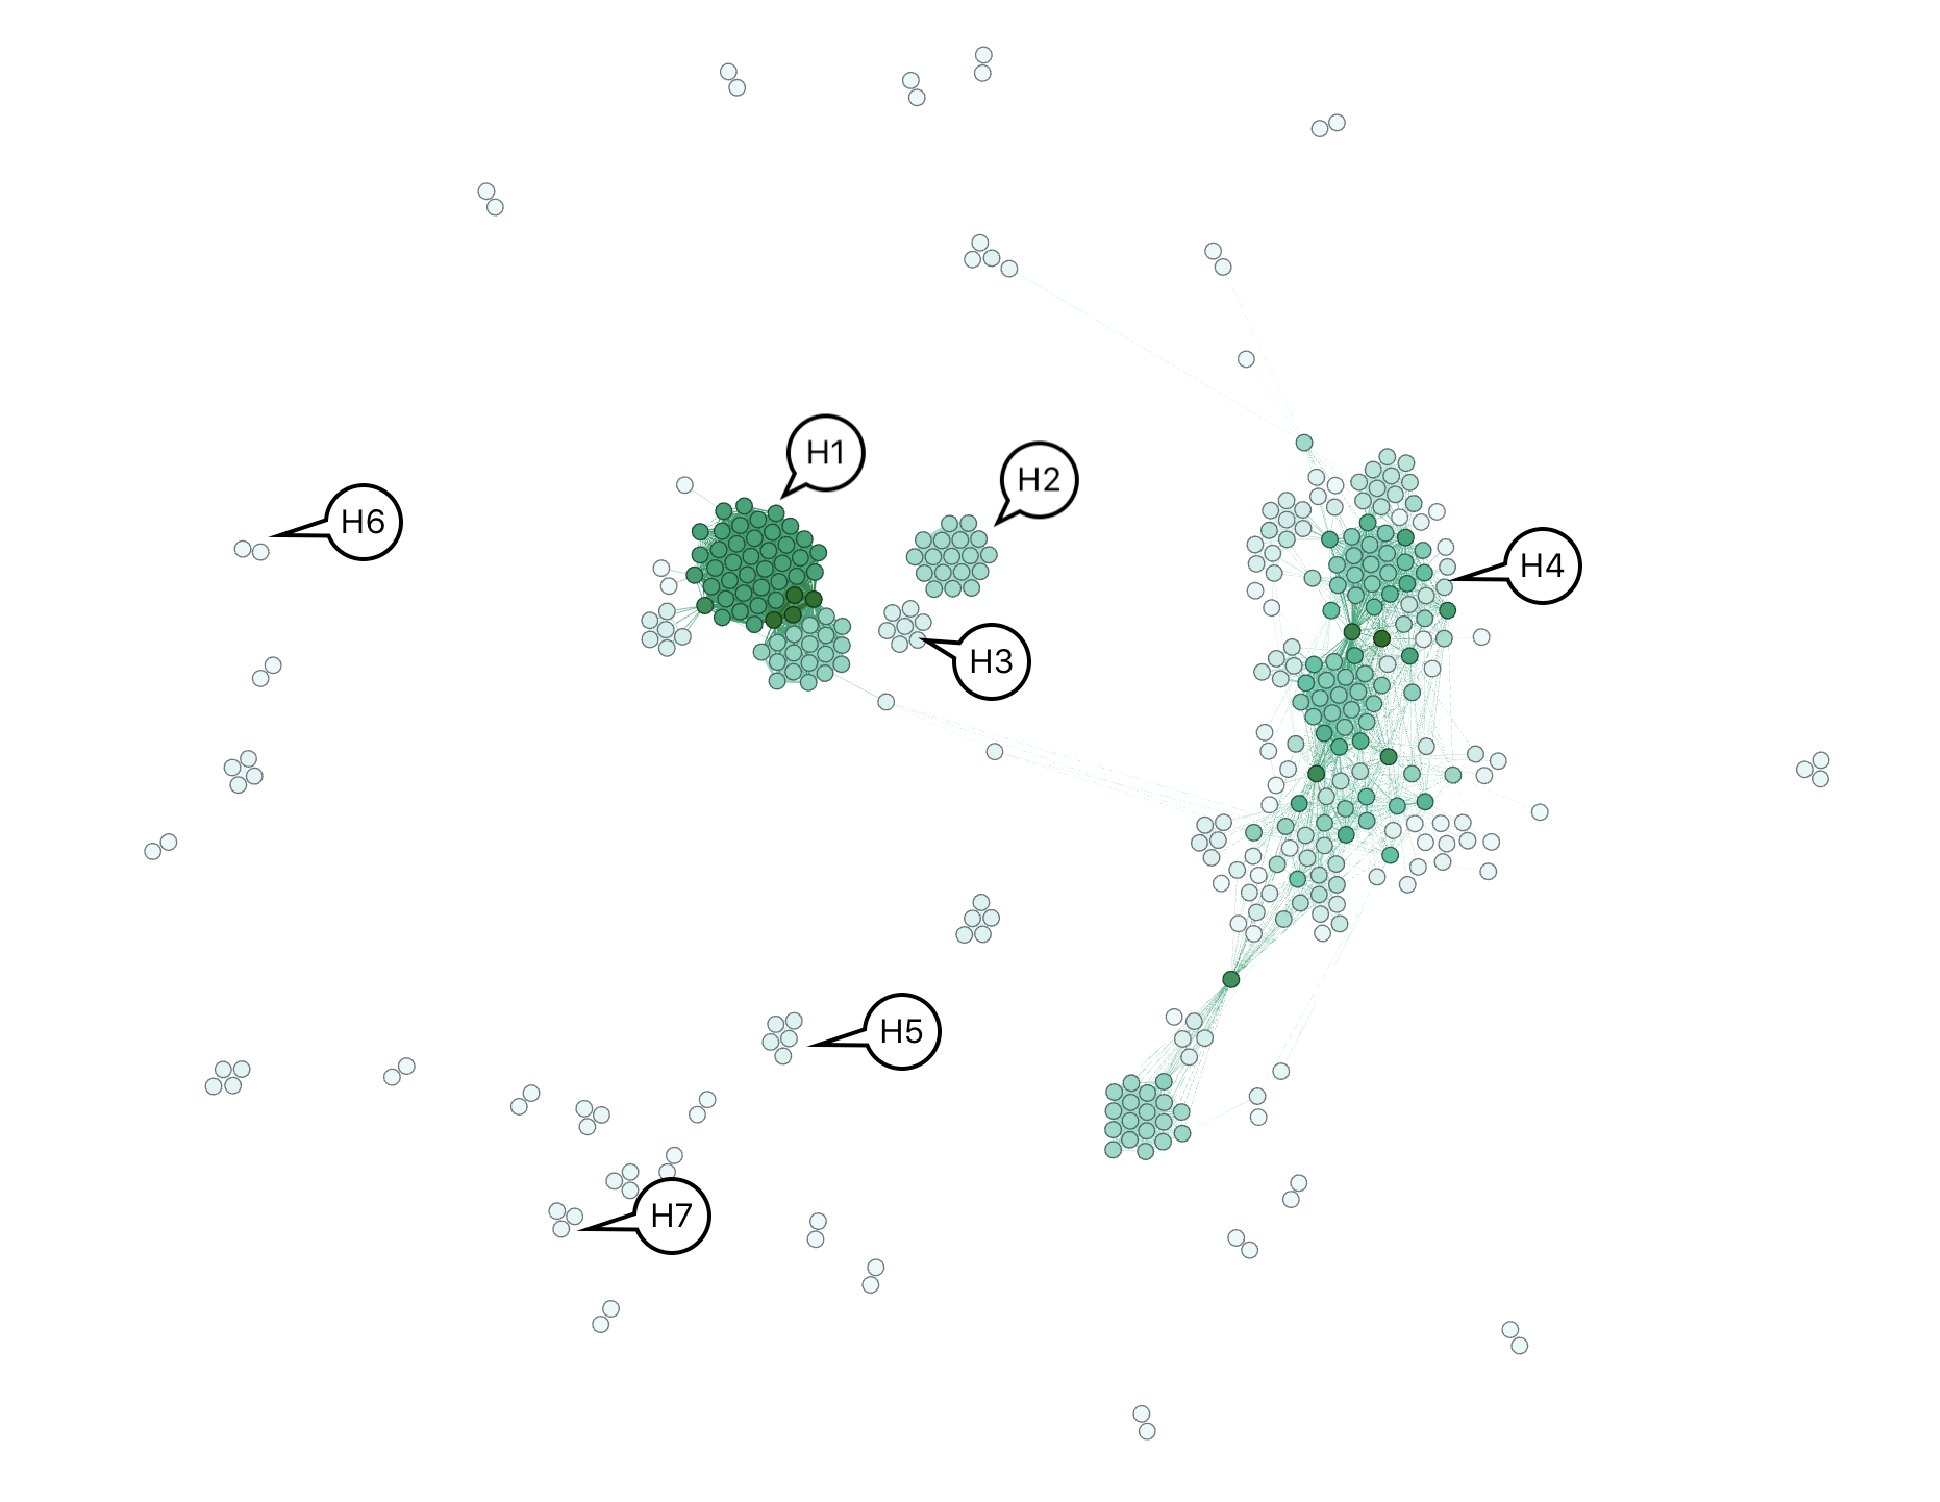
\includegraphics[width=1.0\linewidth]{Thesis/Images/hashtag-sequences-bumbered.pdf}
	\caption{User network built with Hashtag-sequences method}
	\label{fig:hashtag-sequences}
\end{figure}

The suspicious clusters seem to be easy to identify. We consider clusters H1-H5 suspicious and clusters H6-H7 normal. This aligns with the principle based on which we split URL-sharing clusters into suspicious and normal. The tighter a cluster is and the higher node degree is, the more suspicious does the cluster look. 

Surprisingly, the Hashtag-sequences method does not show good results when evaluated on summarised labels. After calculating the key metrics, we have obtained the following results:

\begin{itemize}
    \item Accuracy: 33.33\%;
    \item Precision: 17.65\%;
    \item Recall: 100.00\%.
\end{itemize}

Only the recall metric is high for this method, and it's because the number of False Negative values for this method is zero. The problem of the Hashtag-sequences method is that it labels users as bots way more frequently than needed. Our human respondents labelled most of the ``suspicious'' users as real humans. Therefore, we cannot consider this method reliable and efficient for the task of bot detection in the discourse about the Russian-Ukrainian armed conflict.

\section{Bot influence in the user network}

\subsection{Influentialness}
As can be seen from Table \ref{tab:stats-centrality}, after the removal of potential bot clusters, the centrality metrics distributions have changed significantly. Average degree centrality sinks. Clustering coefficient becomes significantly lower than before the bot removal. 

% Please add the following required packages to your document preamble:
% \usepackage{multirow}
\begin{table}[]
\caption{Comparison of main statistical measures of centrality metrics before and after bot removal}
\label{tab:stats-centrality}
\begin{tabular}{llrrr} \toprule
\textbf{Metric}                         & \textbf{Statistic measure} & \textbf{Full network} & \textbf{Filtered network} & \textbf{Difference} \\ \midrule
\multirow{3}{*}{Degree centrality}      & Mean                       & 0.0034                      & 0.0020                     & 0.0014              \\
                                        & Standard deviation         & 0.0040                      & 0.0013                     & 0.0027              \\
                                        & Maximal value              & 0.0254                      & 0.0051                     & 0.0103              \\
\multirow{3}{*}{Clustering coefficient} & Mean                       & 0.4851                      & 0.4084                     & 0.0767              \\
                                        & Standard deviation         & 0.4848                      & 0.4832                     & 0.0016              \\
                                        & Maximal value              & 1.0000                      & 1.0000                     & 0.0000    \\ \bottomrule         
\end{tabular}
\end{table}

The decrease in centrality metrics and influentialness of the network aligns with the findings of the paper\cite{Hagen2022}; the same behaviour was observed after the removal of bot accounts.

\subsection{Sentiments}
After the potential bots removal, the range of positive, negative and overall sentiment scores becomes more narrow. This can be observed in Table \ref{tab:sentiment-stats}.

% Please add the following required packages to your document preamble:
% \usepackage{multirow}
\begin{table}[]
\caption{Comparison of main statistical measures of sentiment scores before and after bot removal}
\label{tab:sentiment-stats}
\begin{tabular}{llrrr} \toprule
\textbf{Metric}                     & \textbf{Statistic measure} & \multicolumn{1}{l}{\textbf{Full network}} & \multicolumn{1}{l}{\textbf{Filtered network}} & \multicolumn{1}{l}{\textbf{Difference}} \\ \midrule
\multirow{3}{*}{Positive sentiment} & Mean                       & 1.2164                                          & 1.2138                                         & 0.0026                                  \\
                                    & Standard deviation         & 0.4662                                          & 0.4730                                         & -0.0068                                 \\
                                    & Maximal value              & 3.0000                                          & 3.0000                                         & 0.0000                                  \\
\multirow{3}{*}{Negative sentiment} & Mean                       & -1.1973                                         & -1.1775                                        & 0.0198                                  \\
                                    & Standard deviation         & 0.5097                                          & 0.5053                                         & 0.0044                                  \\
                                    & Maximal value              & 0.0000                                          & 0.0000                                         & 0.0000                                  \\
\multirow{3}{*}{Overall sentiment}  & Mean                       & 0.0096                                          & 0.0182                                         & -0.0234                                 \\
                                    & Standard deviation         & 0.1963                                          & 0.1960                                         & 0.0003                                  \\
                                    & Maximal value              & 1.0000                                          & 1.0000                                         & 0.0000     \\ \bottomrule                            
\end{tabular}
\end{table}

The findings of the sentiment analysis suggest that bots influence the sentiments in the user network, primarily by amplifying negative sentiments. They also slightly influence the positive sentiments. This might be explained by the fact that bot creators aim to provoke emotions and emotional decisions among the people reading bot-produced content, to replace the rational thinking with emotions. 


\section{Availability of bot detector to the public}
The screens of the web interface are displayed in Figures \ref{fig:search-screen}, \ref{fig:search-results} and \ref{fig:user-check} 

\begin{figure}
	\centering
	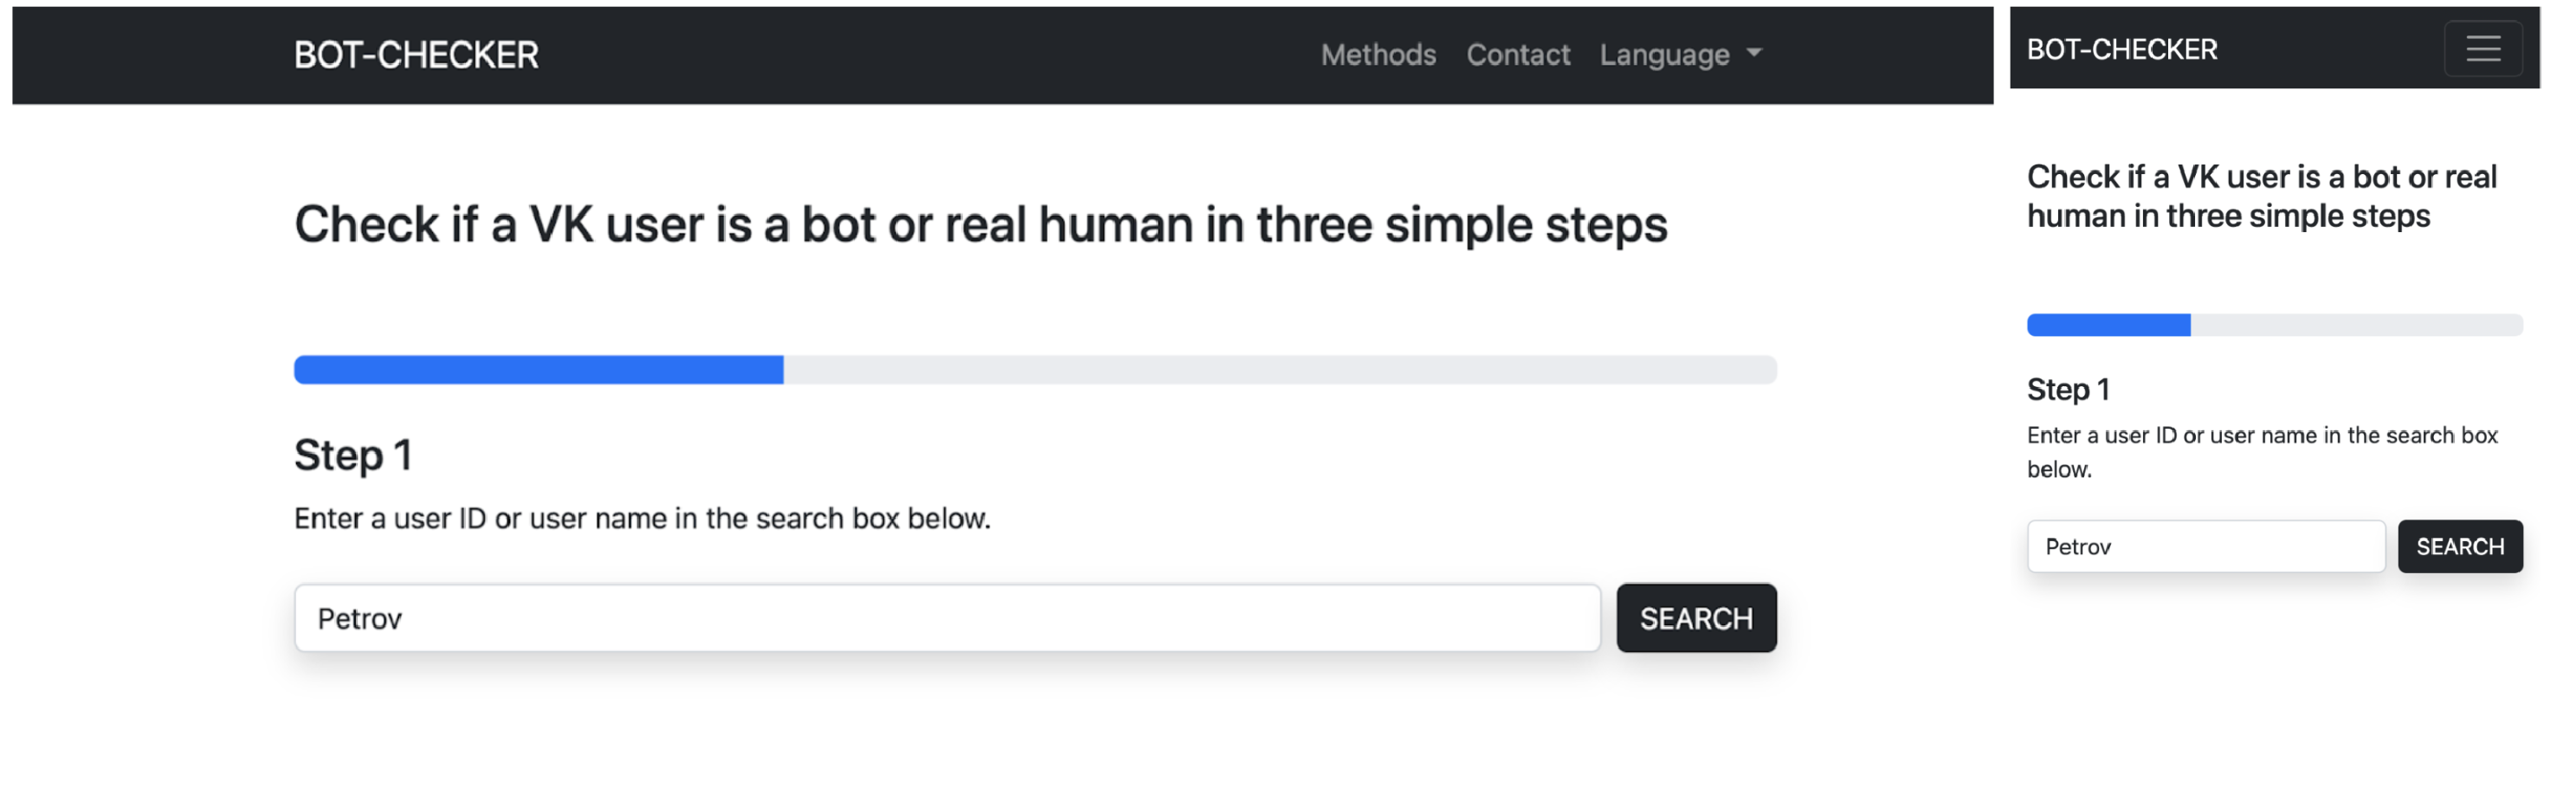
\includegraphics[width=1.0\linewidth]{Thesis/Images/search-screen.pdf}
	\caption{Search screen of the web application, desktop and mobile version}
	\label{fig:search-screen}
\end{figure}

Figure \ref{fig:search-screen} depicts the first step of the user’s journey. This step allows user to type a user ID or first/last name in order to launch a search for a VKontakte user in the database. After pressing the ``Search'' button, a user is redirected to the search results screen (Figure \ref{fig:search-results}).
\begin{figure}
	\centering
	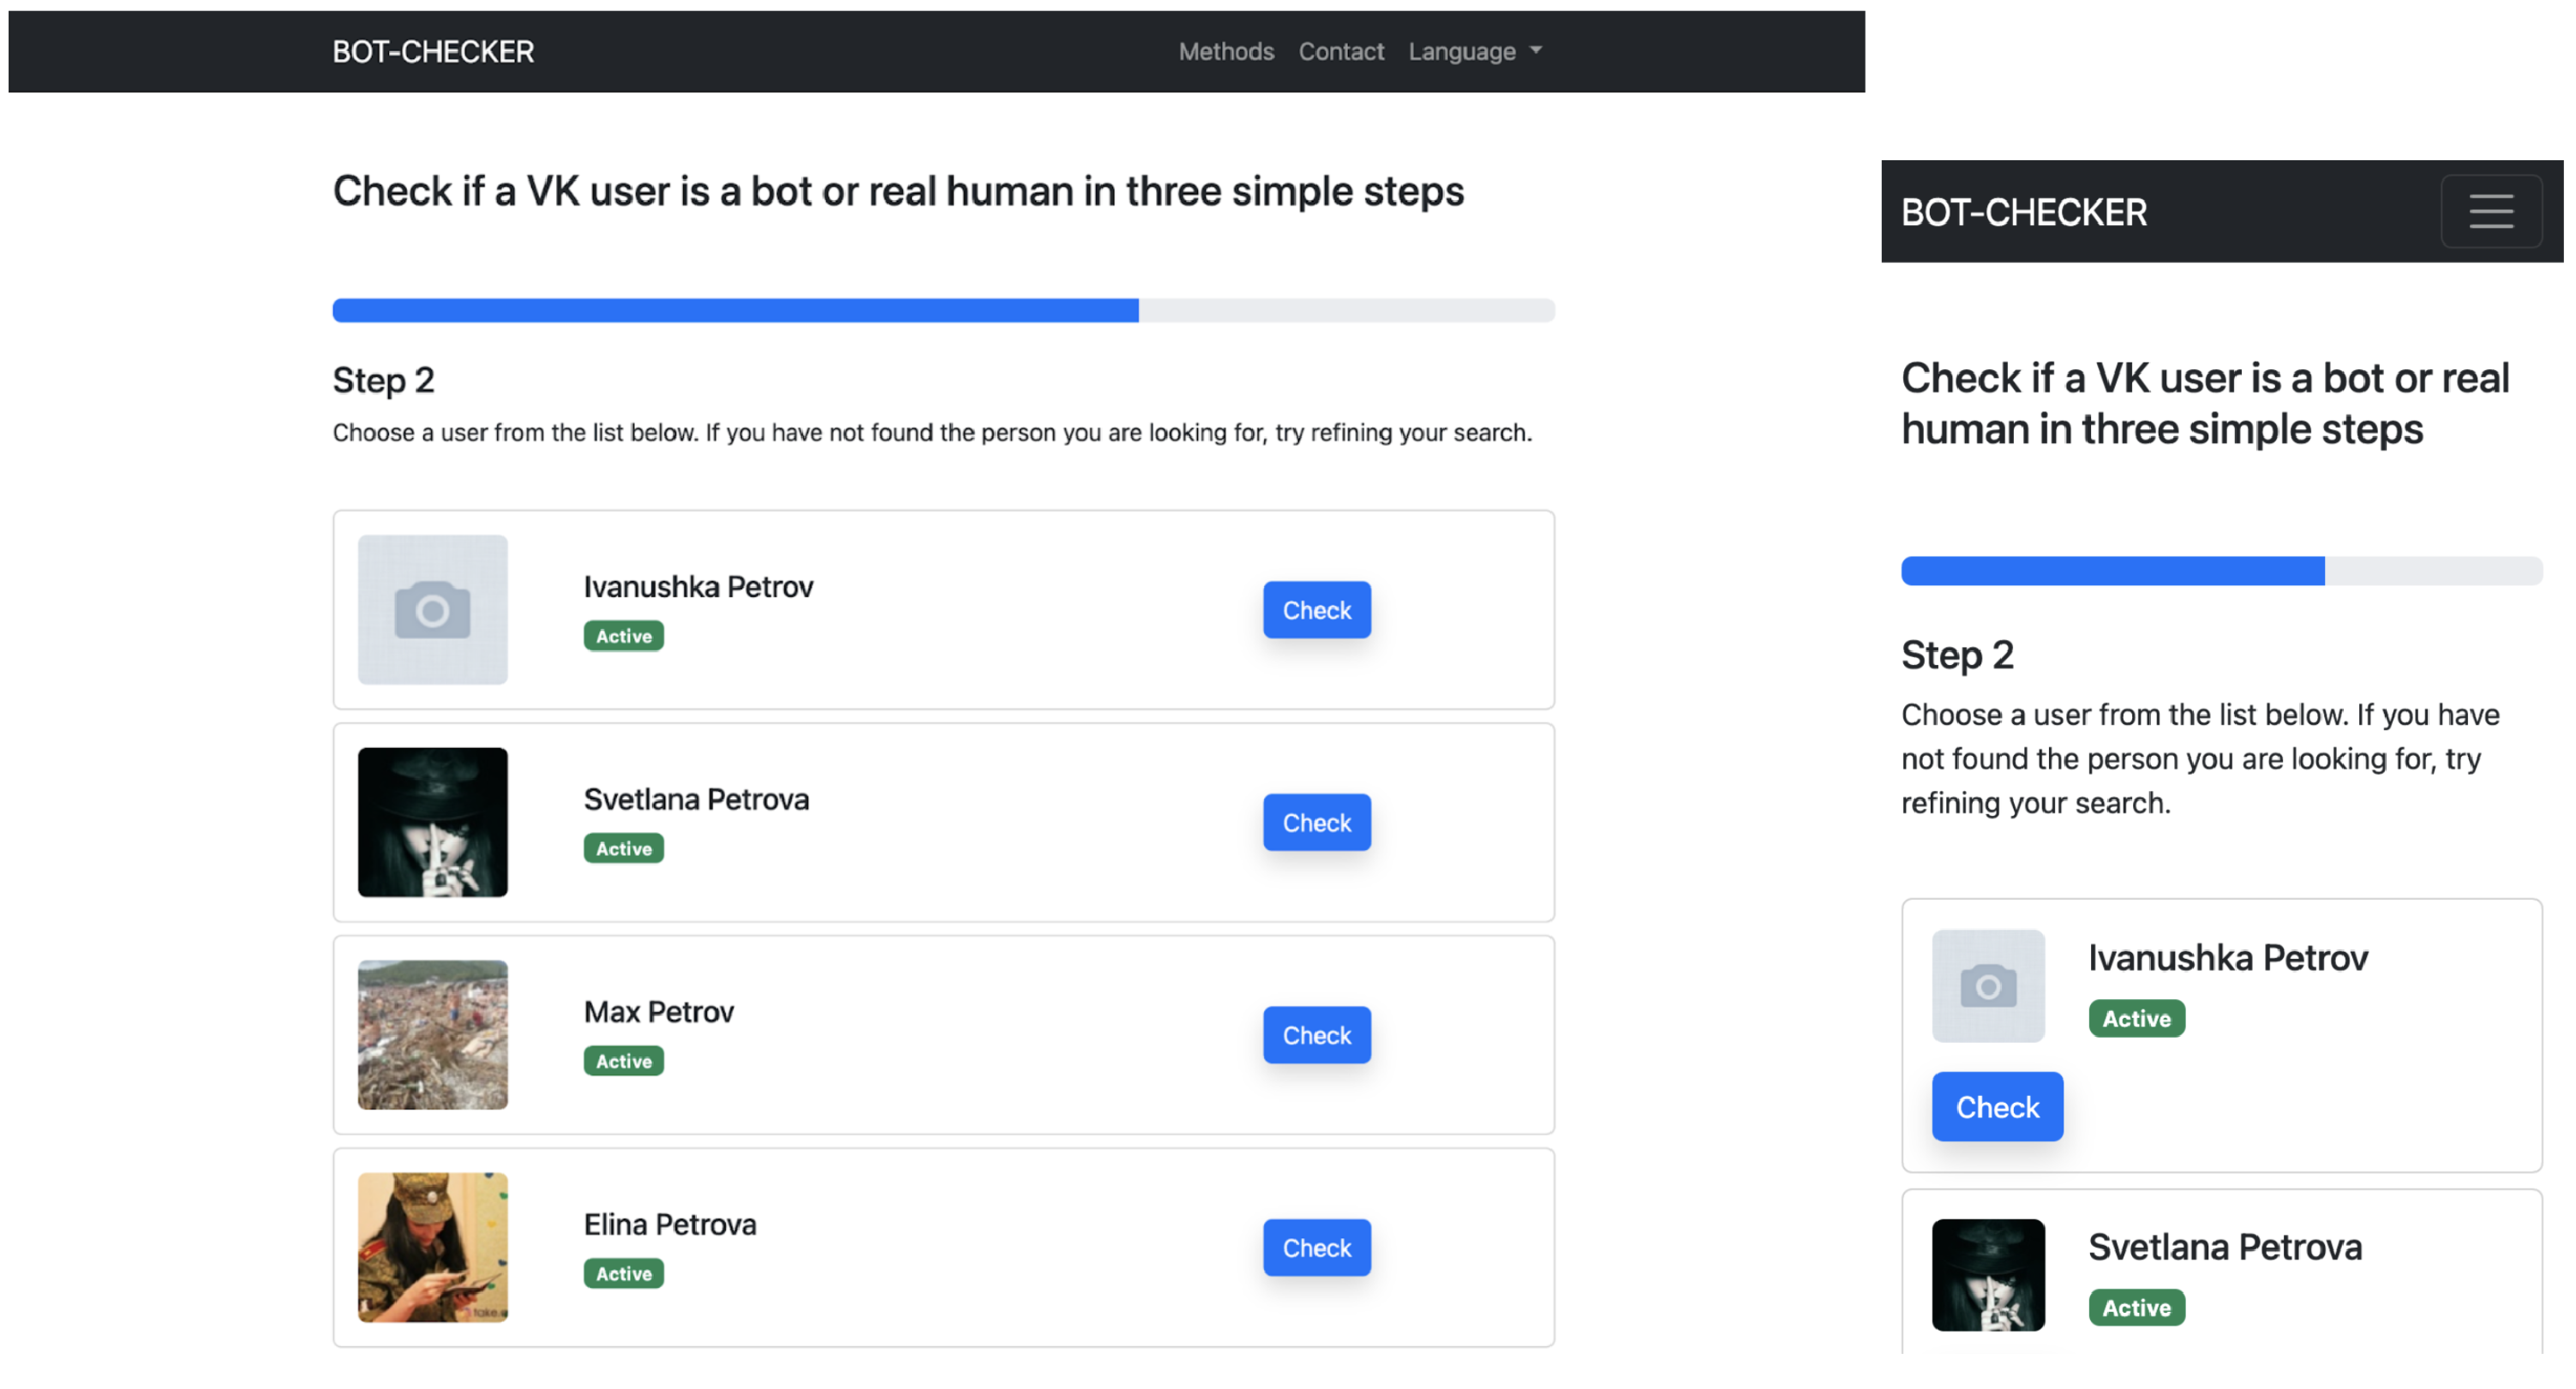
\includegraphics[width=1.0\linewidth]{Thesis/Images/search-results.pdf}
	\caption{Search results screen of the web application, desktop and mobile version}
	\label{fig:search-results}
\end{figure}

In Figure \ref{fig:search-results}, the search results of the query are displayed. The next step for the user is to choose the matching VKontakte user and press ``Check'' to learn if this VKontakte user is a bot, according to our model’s predictions, or not.

\begin{figure}
	\centering
	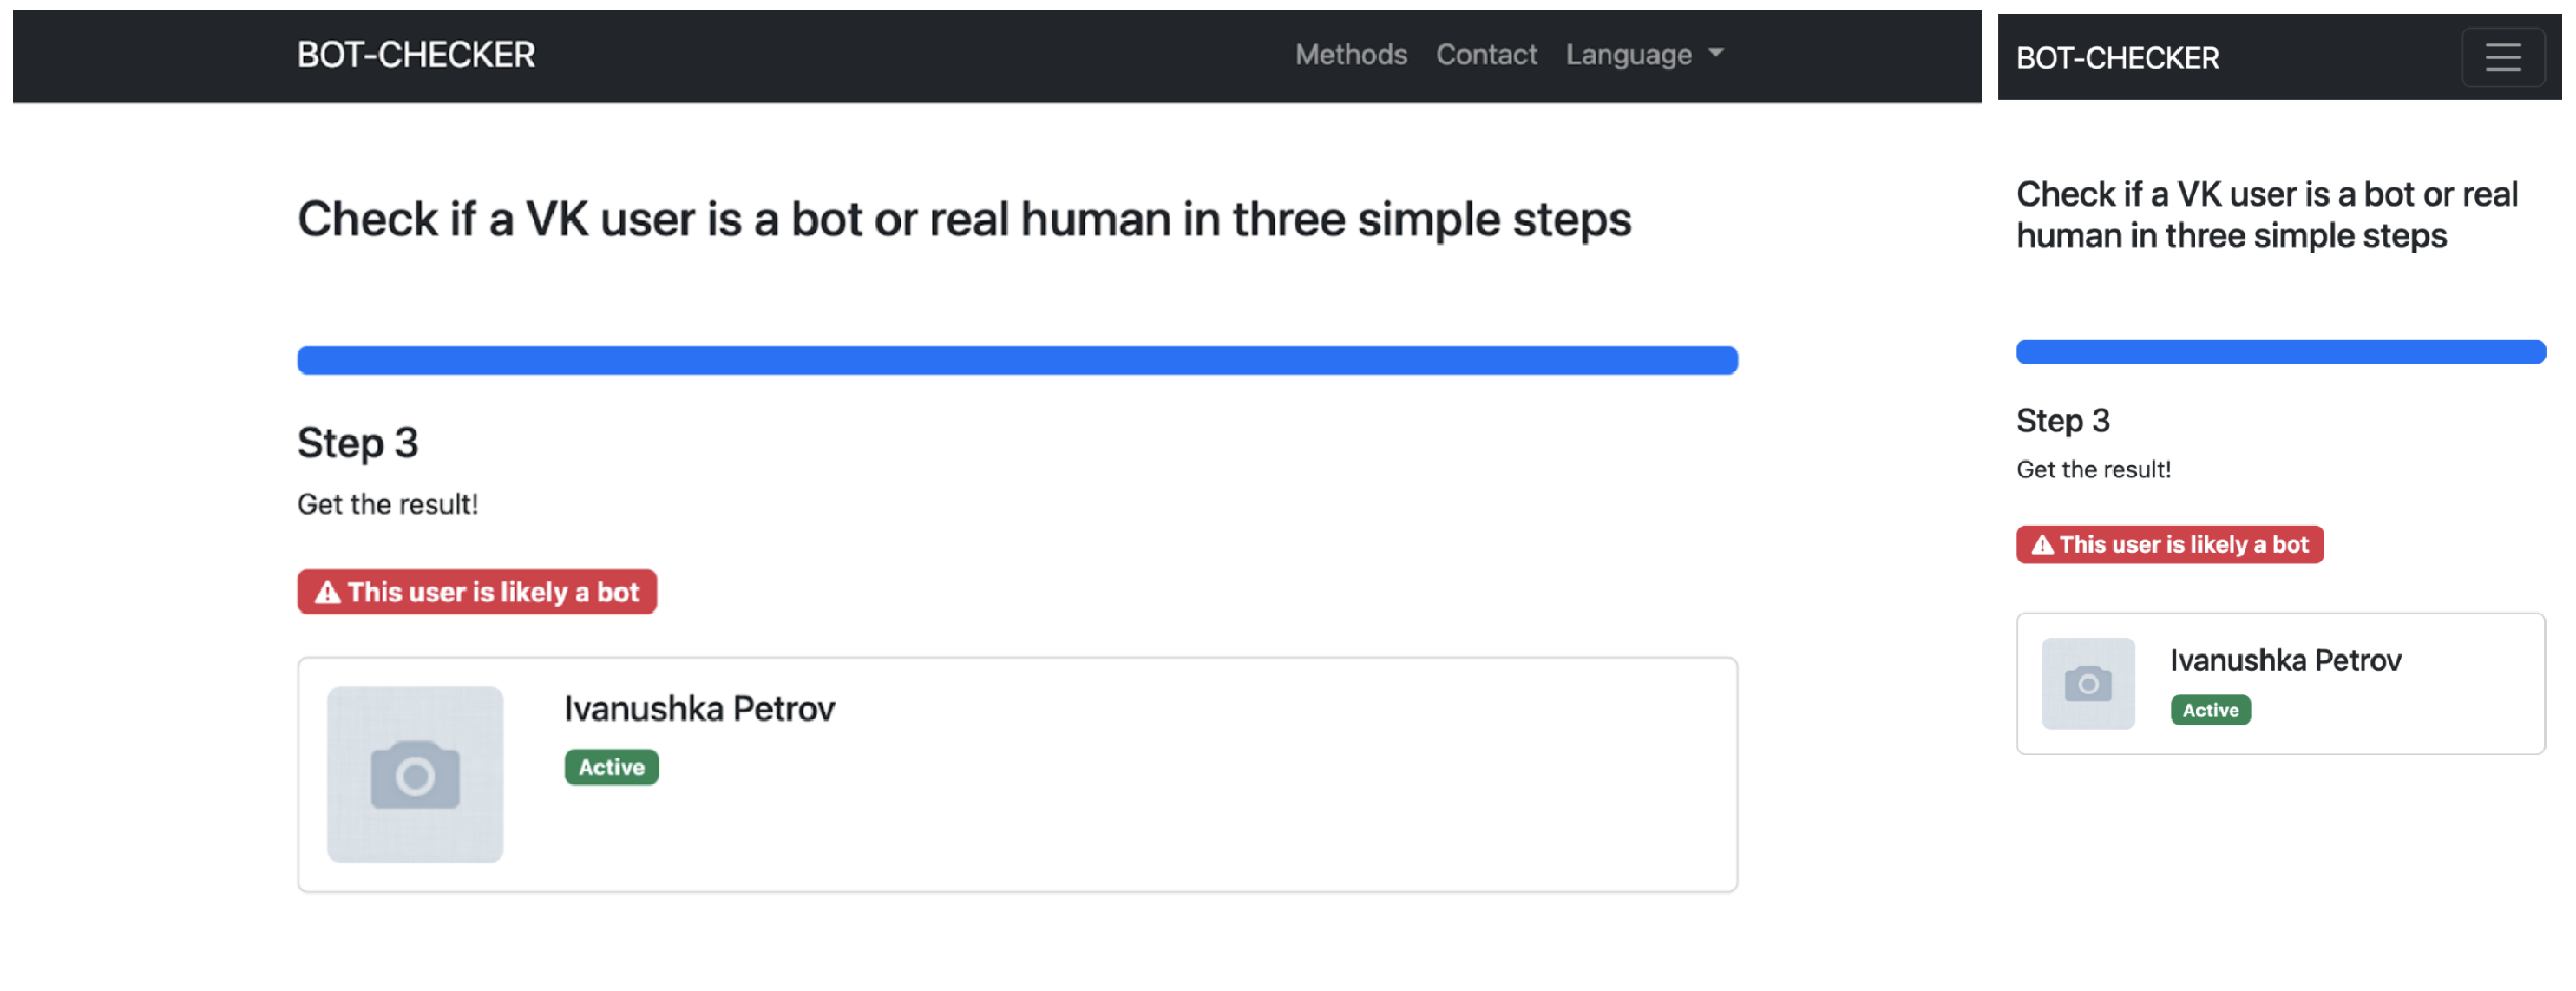
\includegraphics[width=1.0\linewidth]{Thesis/Images/user-check.pdf}
	\caption{User check result screen, desktop and mobile version}
	\label{fig:user-check}
\end{figure}

The last step of the user journey is shown in Figure \ref{fig:user-check} Here, the results of the VKontakte user check are displayed.

The web application presents two other pages: Methods and Contact (Figures \ref{fig:methods-page} and \ref{fig:contact-page}, respectively).

\begin{figure}
	\centering
	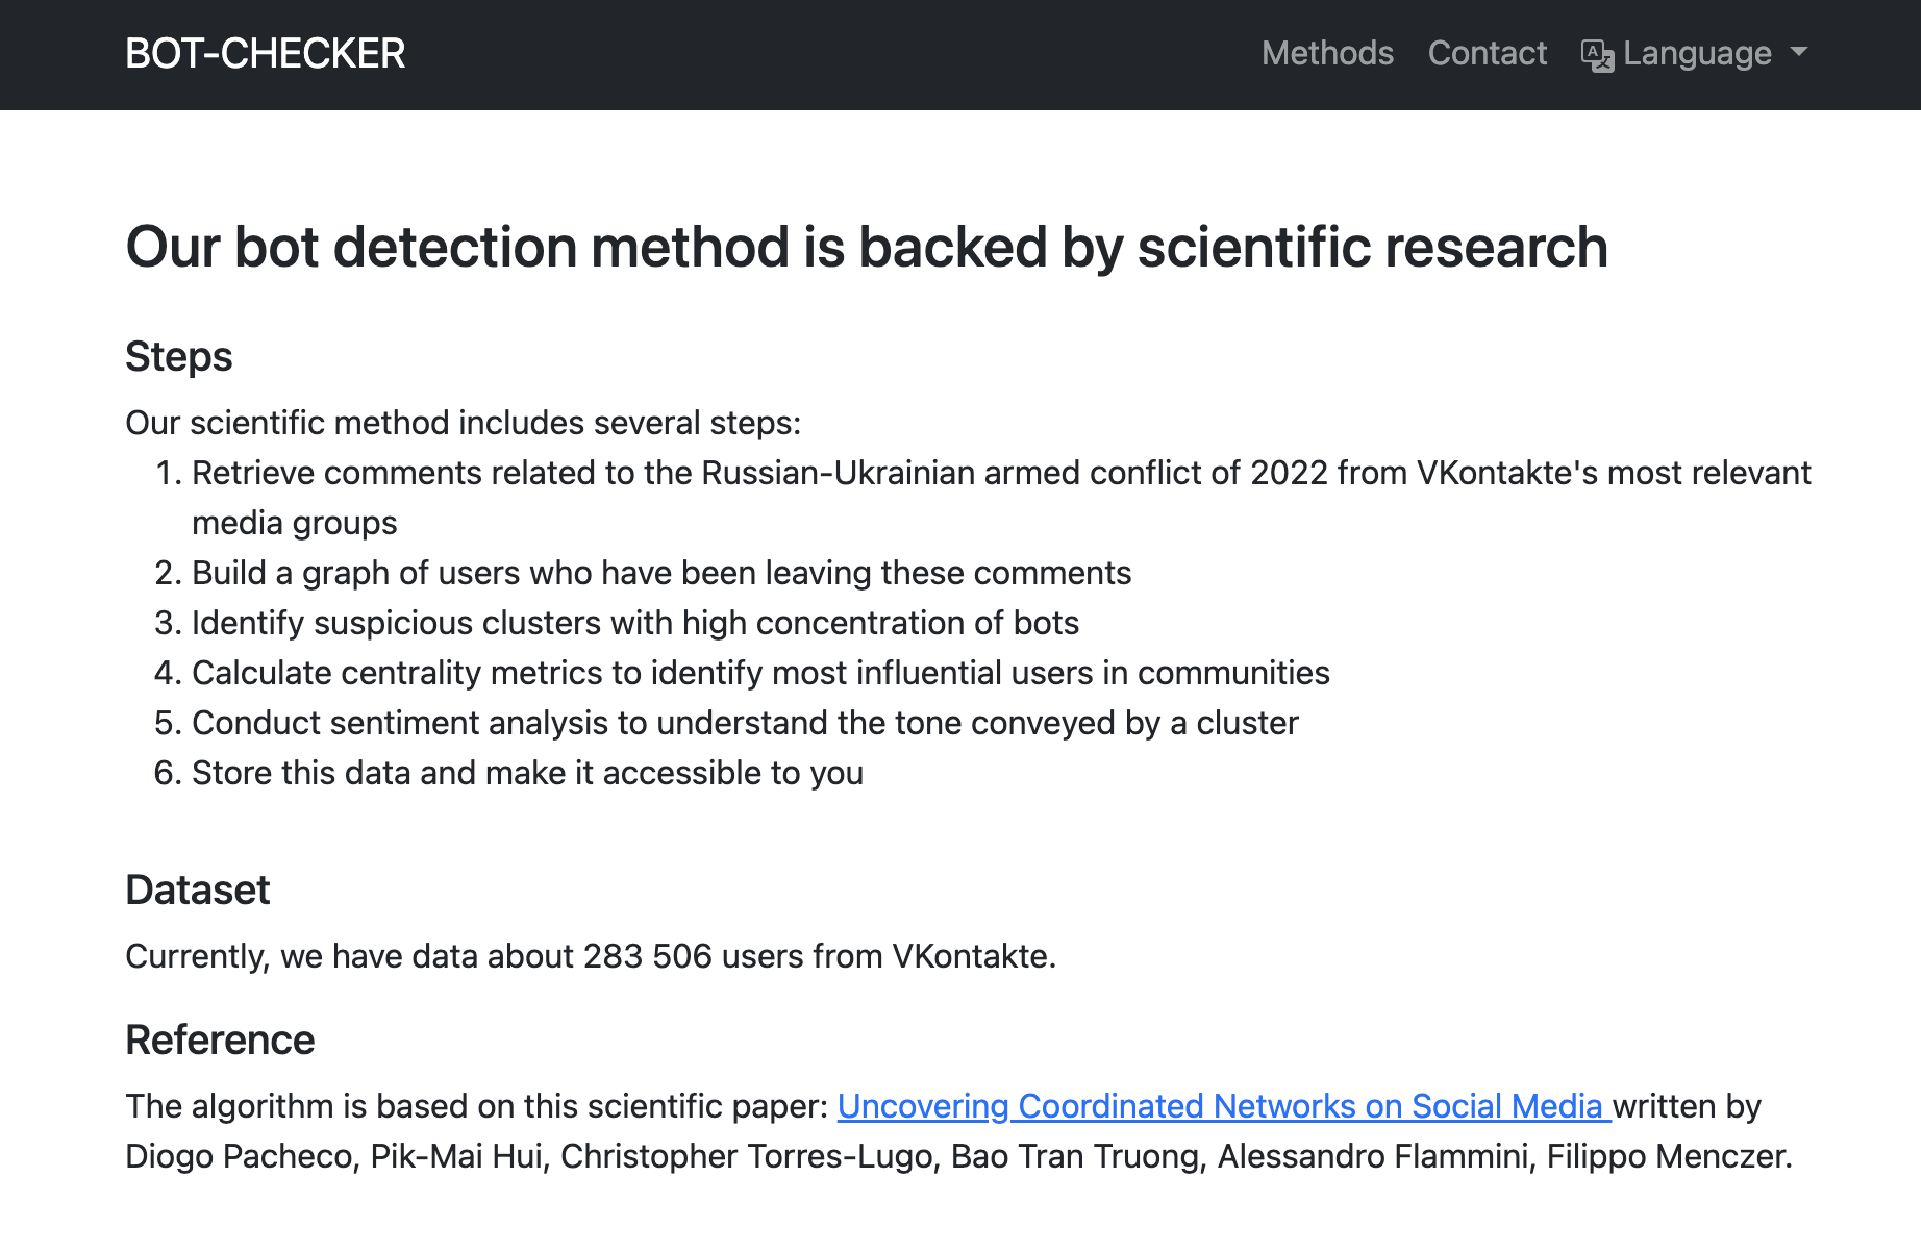
\includegraphics[width=1.0\linewidth]{Thesis/Images/methods-page.pdf}
	\caption{Methods screen, desktop version}
	\label{fig:methods-page}
\end{figure}

The page displayed in Figure \ref{fig:methods-page} gives a top-level overview of the method used for bot detection. Using this page, the user of our system can get acquainted with the technology that lies at the core of the system and sees that the process of bot detection is transparent and based on scientific research.

\begin{figure}
	\centering
	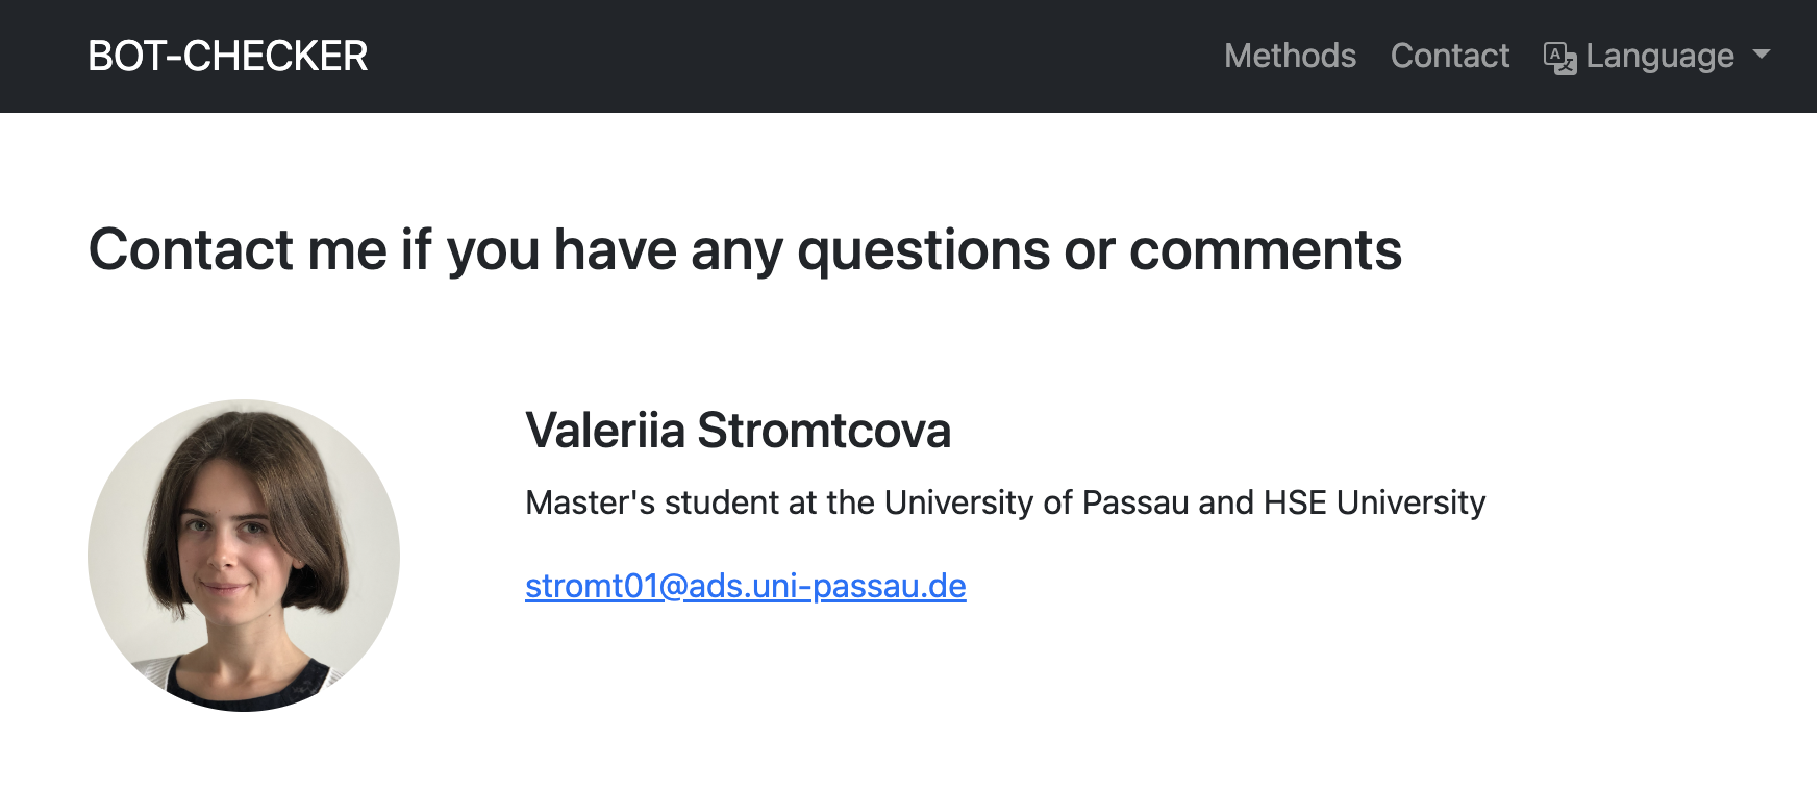
\includegraphics[width=1.0\linewidth]{Thesis/Images/contact-page.pdf}
	\caption{Contact page, desktop version}
	\label{fig:contact-page}
\end{figure}

If a user has any questions, they can use the Contact page depicted in Figure \ref{fig:contact-page}. Here, they can get in touch with the author of this work and ask a question or report a problem. The Methods and Contact page are also responsive to various screen sizes.

Since the system should be multilingual, a language switch control has been implemented. It is available in the header of the website throughout the user journey. The web application is localised with the usage of Babel library\footnote{https://babel.pocoo.org/en/latest/}. An example of the localised interface is given in Figure \ref{fig:localisation}

\begin{figure}
	\centering
	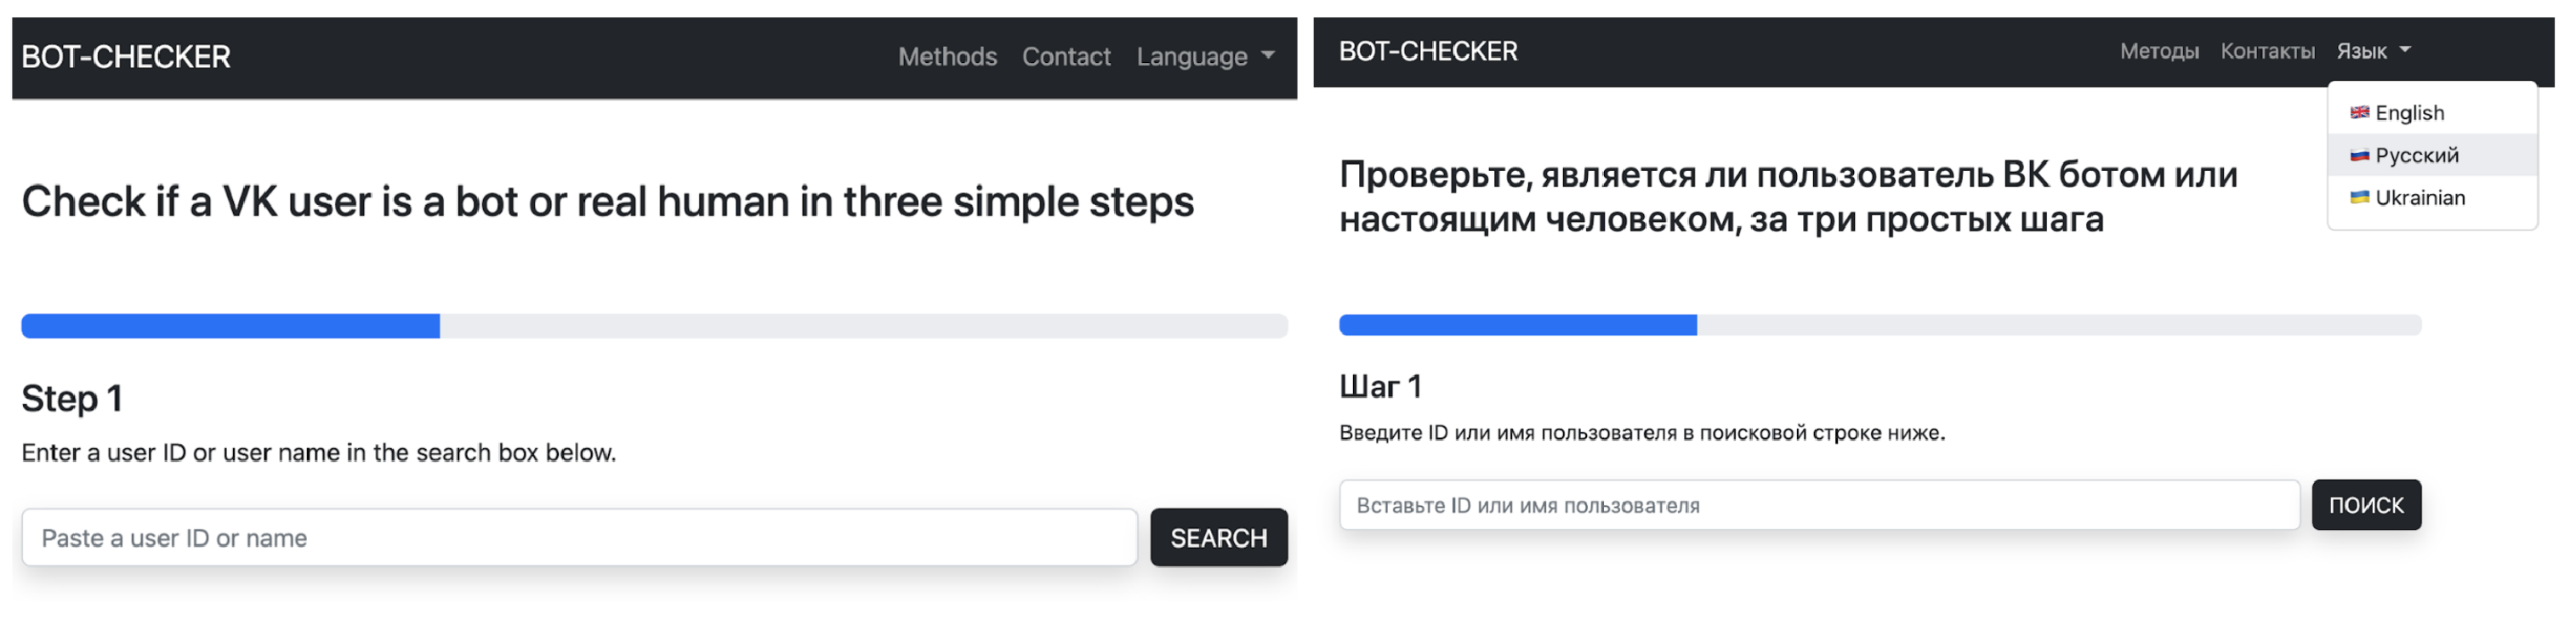
\includegraphics[width=1.0\linewidth]{Thesis/Images/localisation.pdf}
	\caption{Localisation of the search screen, English and Russian versions}
	\label{fig:localisation}
\end{figure}

After the implementation of the web tool, it is necessary to deploy it to a remote server in order to make it accessible to a broad audience. The web application was deployed to a DigitalOcean\footnote{https://www.digitalocean.com/} server. As of March 2023, the system is publicly accessible at the URL address \url{https://bot-detector-x2wo4.ondigitalocean.app/}. The complete source code is available at \url{https://github.com/lerastromtsova/malicious-bot-detection}.

During the web interface implementation and deployment, a system satisfying the functional and non-functional requirements from section \ref{sec:requirements} was built. As a result, any user who has access to the Internet can check if a given VKontakte user is, according to the predictions of our model, a bot or a real person. This can help OSN moderators to more efficiently identify bots, and ordinary users to understand when their opinion is probably being manipulated and uncover this manipulation.
